\chapter{Oxidatie en reductie van alkenen}\label{ch:b2:alkene-redox}

Tweecomponentenepoxylijm zit in twee tubes: de ene bevat moleculen die eindigen op
\omterm{def:b2:alkene-redox:epoxide}{epoxideringen}, drieringen van twee koolstofatomen en een zuurstofatoom; de andere een
amine. Na het mengen gaan de gespannen ringen een voor een open en hardt de pasta uit
tot een stevig netwerk. Alkenen zijn de grondstof van zulke ringen, van alcoholen
op plaatsen waar de regel van Markovnikov ze nooit zou zetten, van diolen met een gekozen
geometrie, en van de kleine fragmenten die chemici vroeger vertelden waar een dubbele
binding in een molecuul lag. Dit hoofdstuk voegt aan de elektrofiele addities van
het deel van jaar~1 de reacties toe die de dubbele binding reduceren of oxideren, en
de stereochemie die elk ervan oplegt.

\begin{recall}
Het deel van jaar~1: elektrofiele addities, regel van Markovnikov, haloniumionen,
syn- en anti-addities, hydratatie van alkenen, oxidatieniveaus van koolstof,
hydridedonoren, chemoselectiviteit, mesoverbindingen en racemische mengsels,
stereospecifieke reacties. \Cref{ch:b2:catalytic-cycles}: de hydrogeneringscyclus van
de katalysator van Wilkinson.
\end{recall}

\begin{omfigure}
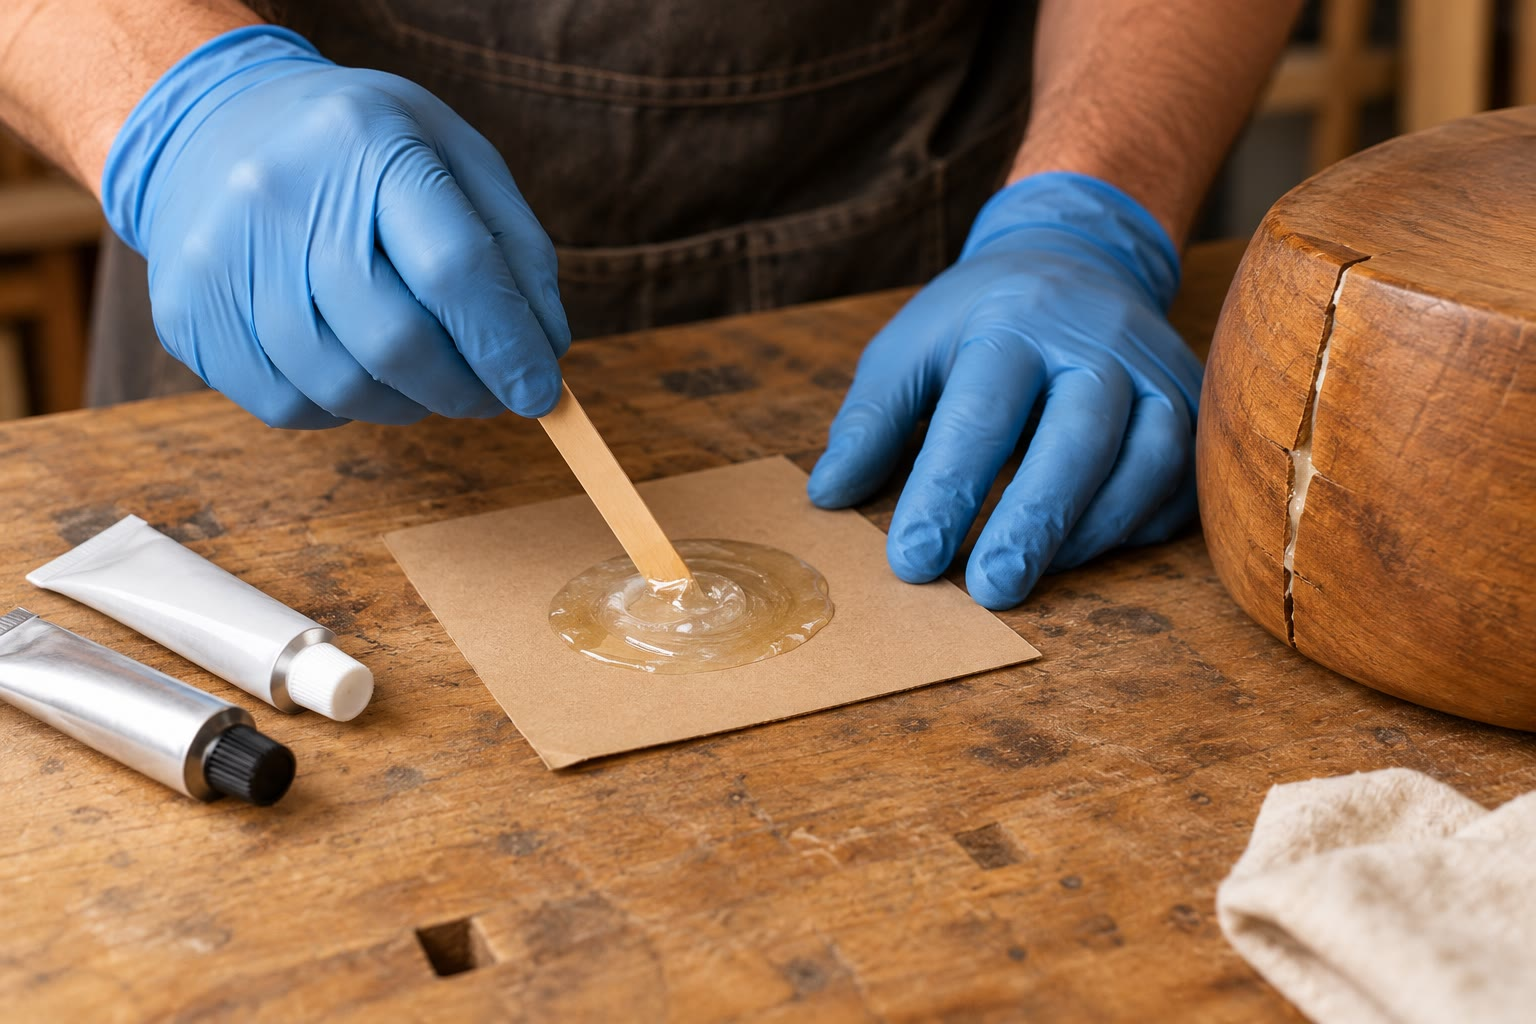
\includegraphics[width=0.6\linewidth]{images/book3/ai/b2-21-epoxy.jpg}

{\small Een tweecomponentenepoxylijm mengen: de hars, met epoxidegroepen, en de
harder, een amine, reageren zodra ze elkaar raken; de ringen gaan open en verbinden de moleculen
tot een vast netwerk.}
\end{omfigure}

\section{Katalytische hydrogenering}

\begin{definition}[Katalytische hydrogenering]\label{def:b2:alkene-redox:hydrogenation}
Een \emph{katalytische hydrogenering}\index{katalytische hydrogenering} addeert diwaterstof aan een
meervoudige binding in aanwezigheid van een katalysator: een fijn verdeeld metaal (palladium op
koolstof, platina, nikkel) bij heterogene katalyse, of een oplosbaar complex zoals
dat van Wilkinson bij homogene katalyse.
\end{definition}

Op een metaaloppervlak worden diwaterstof en het alkeen allebei vastgehouden, de binding \ce{H-H} breekt
tot waterstofatomen aan het oppervlak, en die worden een voor een overgedragen op de koolstofatomen
van het alkeen, dat plat op het metaal ligt.

\begin{proposition}[Syn-additie]\label{prop:b2:alkene-redox:syn-hydrogenation}
\omterm{def:b2:alkene-redox:hydrogenation}{Katalytische hydrogenering} brengt beide waterstofatomen aan op hetzelfde vlak van de dubbele binding.
Een alkyn dat gehydrogeneerd wordt over een vergiftigde palladiumkatalysator stopt bij het alkeen, en dat is het
(\textit{Z})-isomeer.
\end{proposition}

\begin{proof}[Redenering]
Het alkeen is met één vlak aan de katalysator gebonden, en beide waterstofatomen komen van de
katalysator, aan dat vlak: syn-additie. Bij een alkyn staan de twee waterstofatomen die aan de
drievoudige binding geaddeerd worden aan dezelfde kant, cis ten opzichte van elkaar: het (\textit{Z})-alkeen. Een gedeeltelijk
gedeactiveerde katalysator (palladium op calciumcarbonaat met een loodzout en chinoline)
bindt het alkyn veel sterker dan het gevormde alkeen, dat het oppervlak verlaat
vóór een tweede additie.
\end{proof}

\section{Hydroborering--oxidatie}

\begin{definition}[Hydroborering]\label{def:b2:alkene-redox:hydroboration}
Een \emph{hydroborering}\index{hydroborering} addeert een binding B--H van een boraan aan een
binding \ce{C=C}; gevolgd door oxidatie met basisch waterstofperoxide zet ze het
alkeen om in een alcohol waarvan de hydroxylgroep op het minst gesubstitueerde koolstofatoom zit: een
\emph{anti-Markovnikovoriëntatie}\index{anti-Markovnikovorientatie@anti-Markovnikovoriëntatie}.
\end{definition}

\begin{omfigure}
\setchemfig{atom sep=1.8em}
\schemestart[][west]
\chemfig{H_3C-[:30]CH=[:-30]CH_2}
\+ \chemfig{H-BH_2}
\arrow{->[syn-additie]}
\chemfig{H_3C-[:30]CH_2-[:-30]CH_2-[:30]BH_2}
\arrow{->[\ce{H2O2}][\ce{HO-}]}
\chemfig{H_3C-[:30]CH_2-[:-30]CH_2-[:30]OH}
\schemestop
\par\vspace{6pt}

{\small Hydroborering--oxidatie van propeen. Boraan addeert in één stap, boor aan het
eindstandige koolstofatoom en waterstof aan het binnenste, beide aan hetzelfde vlak; oxidatie
vervangt boor door \ce{OH} met behoud van configuratie. Er ontstaat propaan-1-ol, niet het
propaan-2-ol van de zuurgekatalyseerde hydratatie.}
\end{omfigure}

\begin{proposition}[Oriëntatie van de hydroborering]\label{prop:b2:alkene-redox:hydroboration-regio}
Boor addeert aan het minst gesubstitueerde koolstofatoom van de dubbele binding, en waterstof aan het meest
gesubstitueerde; de additie is syn.
\end{proposition}

\begin{proof}[Redenering]
Boor, met een lege p-orbitaal, is het elektrofiel: in de vierkernige overgangstoestand
(de twee koolstofatomen, boor en waterstof) vormt de binding met boor zich iets vóór de binding C--H, en
op het andere koolstofatoom ontstaat een partiële positieve lading, die het meest
gesubstitueerde beter draagt; de omvangrijke boorgroep verkiest ook het minst gehinderde uiteinde. Beide nieuwe bindingen
vormen zich aan één vlak, in een gecoördineerde stap: syn.
\end{proof}

\begin{proposition}[Oxidatie met behoud]\label{prop:b2:alkene-redox:retention}
De oxidatie van een alkylboraan door basisch waterstofperoxide vervangt elke binding C--B door een
binding C--OH met behoud van configuratie aan het koolstofatoom.
\end{proposition}

\begin{proof}[Redenering]
Het hydroperoxide-anion addeert aan boor; een alkylgroep migreert dan van boor naar het
naburige zuurstofatoom, met zijn elektronenpaar, terwijl hydroxide vertrekt; het koolstofatoom houdt zijn bindingen
de hele tijd aan dezelfde kant. Hydrolyse van de binding B--O maakt de alcohol vrij.
\end{proof}

\section{Epoxiden}

\begin{definition}[Epoxide]\label{def:b2:alkene-redox:epoxide}
Een \emph{epoxide}\index{epoxide} (oxiraan) is een cyclische ether met een drieledige ring van
twee koolstofatomen en één zuurstofatoom. Een \emph{epoxidering}\index{epoxidering} zet een alkeen om in
een epoxide, meestal met een \emph{peroxyzuur}\index{peroxyzuur} \ce{RCO3H}, dat
één zuurstofatoom op de dubbele binding overdraagt.
\end{definition}

\begin{omfigure}
\setchemfig{atom sep=2em}
\schemestart
\chemfig{R-[:30]CH=[:-30]CH-[:30]R}
\+ \chemfig{Ar-C(=[2]O)-O-O-H}
\arrow{->}
\chemfig{[:-60]CH(-[:210]R)*3(-CH(-[:-30]R)-O-)}
\+ \chemfig{Ar-C(=[2]O)-OH}
\schemestop
\par\vspace{6pt}

{\small \omterm{def:b2:alkene-redox:epoxide}{Epoxidering} door een \omterm{def:b2:alkene-redox:epoxide}{peroxyzuur} (Ar: bijvoorbeeld een 3-chloorfenylgroep). Het eindstandige
zuurstofatoom van het \omterm{def:b2:alkene-redox:epoxide}{peroxyzuur} wordt in één stap op de dubbele binding overgedragen, waarbij beide bindingen C--O
zich aan hetzelfde vlak vormen.}
\end{omfigure}

\begin{proposition}[Stereospecifieke epoxidering]\label{prop:b2:alkene-redox:epoxidation}
\omterm{def:b2:alkene-redox:epoxide}{Epoxidering} door een \omterm{def:b2:alkene-redox:epoxide}{peroxyzuur} is stereospecifiek: een (\textit{Z})-alkeen geeft het \omterm{def:b2:alkene-redox:epoxide}{cis-epoxide},
een (\textit{E})-alkeen het \omterm{def:b2:alkene-redox:epoxide}{trans-epoxide}.
\end{proposition}

\begin{proof}
Het zuurstofatoom wordt in één gecoördineerde stap overgedragen op één vlak van de dubbele binding, die
intussen niet draait: de onderlinge posities van de substituenten blijven behouden.
\end{proof}

\begin{proposition}[Opening van epoxiden]\label{prop:b2:alkene-redox:opening}
Een nucleofiel opent een \omterm{def:b2:alkene-redox:epoxide}{epoxide} door aanval op één koolstofatoom vanaf het vlak tegenover het zuurstofatoom
(anti-opening, met inversie aan dat koolstofatoom). Onder basische omstandigheden valt het het minst
gehinderde koolstofatoom aan; onder zure omstandigheden het meest gesubstitueerde.
\end{proposition}

\begin{proof}[Redenering]
De ringspanning maakt de bindingen C--O gemakkelijk te verbreken. Met een sterk nucleofiel en zonder zuur
is de opening een bimoleculaire substitutie, en het minst gehinderde koolstofatoom is het
gemakkelijkst bereikbaar. In zuur wordt het zuurstofatoom geprotoneerd; de binding C--O met het meest gesubstitueerde koolstofatoom
rekt het sterkst uit, want dat koolstofatoom draagt de grootste partiële positieve lading, en zelfs een zwak
nucleofiel (water, een alcohol) valt daar aan --- nog steeds van achteren, dus nog steeds anti.
\end{proof}

\begin{omfigure}
\setchemfig{atom sep=2em}
\schemestart
\chemfig{[:-60]C(-[:210]H_3C)(-[:150]H_3C)*3(-CH_2-O-)}
\arrow{->[\ce{CH3O-}][\ce{CH3OH}]}[,1.4]
\chemfig{H_3C-C(-[2]CH_3)(-[6]OH)-CH_2-OCH_3}
\schemestop

\medskip
\schemestart
\chemfig{[:-60]C(-[:210]H_3C)(-[:150]H_3C)*3(-CH_2-O-)}
\arrow{->[\ce{CH3OH}][\ce{H+}]}[,1.4]
\chemfig{H_3C-C(-[2]CH_3)(-[6]OCH_3)-CH_2-OH}
\schemestop
\par\vspace{6pt}

{\small Opening van 2,2-dimethyloxiraan door methanol. Boven, met methoxide: aanval op de
\ce{CH2}, het minst gehinderde koolstofatoom. Onder, in zuur: aanval op het meest gesubstitueerde koolstofatoom,
dat het grootste deel van de positieve lading van het geprotoneerde \omterm{def:b2:alkene-redox:epoxide}{epoxide} draagt.}
\end{omfigure}

\section{Dihydroxylering}

\begin{definition}[Dihydroxylering]\label{def:b2:alkene-redox:dihydroxylation}
Een \emph{dihydroxylering}\index{dihydroxylering} zet een alkeen om in een 1,2-diol door
één \ce{OH}-groep aan elk koolstofatoom van de dubbele binding toe te voegen.
\end{definition}

Osmiumtetroxide, in katalytische hoeveelheid met een heroxidator, en koud verdund permanganaat brengen
beide zuurstofatomen aan via een cyclische ester, aan één vlak: een \omterm{def:b2:alkene-redox:dihydroxylation}{syn-dihydroxylering}. \omterm{def:b2:alkene-redox:epoxide}{Epoxidering}
gevolgd door opening met water in zuur geeft het anti-diol.

\begin{proposition}[Syn- en anti-diolen]\label{prop:b2:alkene-redox:diols}
Uit (\textit{Z})-but-2-een geeft \omterm{def:b2:alkene-redox:dihydroxylation}{syn-dihydroxylering} meso-butaan-2,3-diol en de epoxideroute
geeft de racemische (2\textit{R},3\textit{R})- en (2\textit{S},3\textit{S})-diolen; uit
(\textit{E})-but-2-een zijn de resultaten omgewisseld.
\end{proposition}

\begin{proof}
In (\textit{Z})-but-2-een staan de twee methylgroepen aan dezelfde kant. Twee \ce{OH} aan één vlak toevoegen
geeft een diol waarin, getekend in de eclipsconformatie van de vroegere dubbele binding, de
twee \ce{OH} aan de ene kant staan en de twee methylgroepen aan de andere: een spiegelvlak loopt tussen
C2 en C3, de mesoverbinding. De epoxideroute zet de twee \ce{OH} aan tegenovergestelde vlakken
(anti): het spiegelvlak verdwijnt, en de aanval op elk van beide koolstofatomen van het achirale \omterm{def:b2:alkene-redox:epoxide}{epoxide},
even waarschijnlijk, geeft de twee enantiomeren in gelijke hoeveelheden. Bij het (\textit{E})-alkeen verandert elke
stap de verhouding van de methylgroepen, wat de uitkomsten omwisselt.
\end{proof}

\begin{omfigure}
\begin{tikzpicture}[font=\small]
  \begin{scope}
    \draw[thick] (0,0) -- (0,1.2);
    \draw[thick] (0,1.2) -- (-0.7,1.45); \draw[thick] (0,1.2) -- (0.7,1.45);
    \node[anchor=east] at (-0.7,1.45) {\ce{HO}}; \node[anchor=west] at (0.7,1.45) {\ce{CH3}};
    \draw[thick] (0,0) -- (-0.7,0.25); \draw[thick] (0,0) -- (0.7,0.25);
    \node[anchor=east] at (-0.7,0.25) {\ce{HO}}; \node[anchor=west] at (0.7,0.25) {\ce{CH3}};
    \node[anchor=south] at (0,1.25) {\scriptsize H};
    \node[anchor=north] at (0,-0.05) {\scriptsize H};
    \draw[densely dashed, omThm] (-1.6,0.6) -- (1.6,0.6);
    \node at (0,-1.0) {syn: meso};
  \end{scope}
  \begin{scope}[xshift=6.5cm]
    \draw[thick] (0,0) -- (0,1.2);
    \draw[thick] (0,1.2) -- (-0.7,1.45); \draw[thick] (0,1.2) -- (0.7,1.45);
    \node[anchor=east] at (-0.7,1.45) {\ce{HO}}; \node[anchor=west] at (0.7,1.45) {\ce{CH3}};
    \draw[thick] (0,0) -- (-0.7,0.25); \draw[thick] (0,0) -- (0.7,0.25);
    \node[anchor=east] at (-0.7,0.25) {\ce{H3C}}; \node[anchor=west] at (0.7,0.25) {\ce{OH}};
    \node[anchor=south] at (0,1.25) {\scriptsize H};
    \node[anchor=north] at (0,-0.05) {\scriptsize H};
    \node[align=center] at (0,-1.1) {anti: één enantiomeer\\ (gevormd met zijn spiegelbeeld)};
  \end{scope}
\end{tikzpicture}

{\small De twee butaan-2,3-diolen uit (\textit{Z})-but-2-een, schematisch (verticale binding C2--C3,
de twee groepen van elk koolstofatoom links en rechts getekend). Syn-additie zet beide
\ce{OH} aan dezelfde kant: een intern spiegelvlak (gestreept), de mesoverbinding. Anti-additie
zet ze aan tegenovergestelde kanten: een chiraal diol, gevormd samen met zijn enantiomeer.}
\end{omfigure}

\section{Oxidatieve splitsing}

\begin{definition}[Oxidatieve splitsing]\label{def:b2:alkene-redox:cleavage}
Een \emph{oxidatieve splitsing}\index{oxidatieve splitsing} verbreekt beide bindingen van een dubbele
binding \ce{C=C} en maakt van elk koolstofatoom een carbonyl- of carboxylgroep. Bij een
\emph{ozonolyse}\index{ozonolyse} reageert het alkeen met ozon en wordt het intermediaire
ozonide in een tweede stap ontleed, de opwerking.
\end{definition}

\begin{proposition}[Producten van ozonolyse]\label{prop:b2:alkene-redox:ozonolysis}
\omterm{def:b2:alkene-redox:cleavage}{Ozonolyse} splitst elke binding \ce{C=C} in twee groepen \ce{C=O}. Met een reductieve opwerking
(zink en zuur, of dimethylsulfide) geeft een koolstofatoom dat een waterstofatoom draagt een aldehyde; met
een oxidatieve opwerking (waterstofperoxide) geeft het een carbonzuur. Een koolstofatoom met twee
koolstofgroepen geeft in beide gevallen een keton.
\end{proposition}

\begin{proof}[Redenering]
Ozon addeert aan de dubbele binding, het intermediair lagert om en de binding C--C breekt, wat
een ozonide geeft waarin elk vroeger alkeenkoolstofatoom aan twee zuurstofatomen gebonden is. De opwerking reduceert het
tot twee carbonylverbindingen, of oxideert de aldehyden verder. De tussenstappen worden
aangenomen.
\end{proof}

\begin{omfigure}
\setchemfig{atom sep=2em}
\schemestart
\chemfig{H_3C-[:30]C(-[:90]CH_3)=[:-30]CH-[:30]CH_3}
\arrow{->[1. \ce{O3}][2. \ce{Zn}, \ce{H+}]}[,1.8]
\chemfig{H_3C-C(=[2]O)-CH_3}
\+
\chemfig{H-C(=[2]O)-CH_3}
\schemestop
\par\vspace{6pt}

{\small \omterm{def:b2:alkene-redox:cleavage}{Ozonolyse} van 2-methylbut-2-een met een reductieve opwerking: propanon en
ethanal. Wie de twee carbonylkoolstofatomen opnieuw met een dubbele binding verbindt, krijgt het
alkeen terug.}
\end{omfigure}

\begin{method}[Een dubbele binding lokaliseren]\label{met:b2:alkene-redox:locate-double-bond}
\begin{enumerate}
  \item Som de carbonylfragmenten van de \omterm{def:b2:alkene-redox:cleavage}{ozonolyse} op en tel hun koolstofatomen; samen moeten ze
        het aantal van het alkeen geven.
  \item Elk koolstofatoom van een \ce{C=O} was een dubbel gebonden koolstofatoom: verbind de fragmenten door twee
        \ce{C=O} te vervangen door één \ce{C=C}.
  \item Bij een ring komt er één molecuul met twee carbonylgroepen uit; verbind de twee uiteinden ervan.
  \item Controleer met de formule en de onverzadigingsgraad.
\end{enumerate}
\end{method}

Heet geconcentreerd permanganaat splitst ook dubbele bindingen, en geeft zuren en ketonen; natriumperiodaat
splitst 1,2-diolen in twee carbonylverbindingen, een mildere route via het diol.

\begin{method}[Een reagens kiezen voor een alkeen]\label{met:b2:alkene-redox:choose-reagent}
\begin{center}
\small
\renewcommand{\arraystretch}{1.15}
\begin{tabular}{lll}
doel & reagens & stereochemie, oriëntatie \\ \hline
alkaan & \ce{H2}, Pd/C & syn \\
Markovnikov-alcohol & \ce{H2O}, zuur & via een carbokation \\
anti-Markovnikov-alcohol & \ce{BH3}, dan \ce{H2O2}, \ce{HO-} & syn \\
\omterm{def:b2:alkene-redox:epoxide}{epoxide} & \omterm{def:b2:alkene-redox:epoxide}{peroxyzuur} & stereospecifiek \\
syn-diol & \ce{OsO4} (kat.) of koud \ce{MnO4-} & syn \\
anti-diol & \omterm{def:b2:alkene-redox:epoxide}{peroxyzuur}, dan \ce{H2O}, zuur & anti \\
twee carbonylen & \ce{O3}, dan \ce{Zn}/zuur & splitsing \\
\end{tabular}
\end{center}
\end{method}

\begin{safety}{\ghs[5mm]{GHS02}\,\ghs[5mm]{GHS03}\,\ghs[5mm]{GHS05}\,\ghs[5mm]{GHS06}}
Osmiumtetroxide is vluchtig en zeer giftig (het beschadigt de ogen); het wordt in katalytische
hoeveelheid in oplossing gebruikt, in een zuurkast. \omterm{def:b2:alkene-redox:epoxide}{Peroxyzuren} en waterstofperoxide zijn oxidatoren die
heftig kunnen ontleden bij verhitting of in geconcentreerde vorm; boraanoplossingen zijn ontvlambaar;
ozon is giftig en wordt in een zuurkast gegenereerd.
% ledger: ghs:OsO4, ghs:mCPBA, ghs:BH3-THF, ghs:O3, ghs:NaIO4
\end{safety}

\section{Oefeningen}

\begin{exercise}[$\star$]\label{exo:b2:alkene-redox:1}
Geef het product van 1-methylcyclohexeen met: \ce{H2}/Pd; \ce{H2O}/\ce{H+};
\ce{BH3} dan \ce{H2O2}/\ce{HO-}; een \omterm{def:b2:alkene-redox:epoxide}{peroxyzuur}; \ce{OsO4} (kat.); \ce{O3} dan
\ce{Zn}/\ce{H+}.
\end{exercise}

\begin{exercise}[$\star$]\label{exo:b2:alkene-redox:2}
Welke alcohol geeft hydroborering--oxidatie uit 2-methylpropeen? En zuurgekatalyseerde
hydratatie?
\end{exercise}

\begin{exercise}[$\star$]\label{exo:b2:alkene-redox:3}
Teken het \omterm{def:b2:alkene-redox:epoxide}{epoxide} dat uit (\textit{E})-but-2-een gevormd wordt. Is het chiraal?
\end{exercise}

\begin{exercise}[$\star$]\label{exo:b2:alkene-redox:4}
Geef de producten van de \omterm{def:b2:alkene-redox:cleavage}{ozonolyse} van hex-3-een met een reductieve opwerking, en daarna met een
oxidatieve opwerking.
\end{exercise}

\begin{exercise}[$\star\star$]\label{exo:b2:alkene-redox:5}
Geef de diolen die gevormd worden uit (\textit{Z})-but-2-een (a) met \ce{OsO4}; (b) met een \omterm{def:b2:alkene-redox:epoxide}{peroxyzuur}
en daarna waterig zuur. Welk ervan is optisch inactief omdat het meso is, en welk
omdat het racemisch is?
\end{exercise}

\begin{exercise}[$\star\star$]\label{exo:b2:alkene-redox:6}
2,2-Dimethyloxiraan wordt geopend door water in zuur en door hydroxide. Geven de twee routes
hetzelfde product? Leg uit.
\end{exercise}

\begin{exercise}[$\star\star$]\label{exo:b2:alkene-redox:7}
Hoe zou je (\textit{Z})-hex-3-een bereiden uit hex-3-yn?
\end{exercise}

\begin{exercise}[$\star\star$]\label{exo:b2:alkene-redox:8}
Een alkeen \ce{C7H14} geeft bij \omterm{def:b2:alkene-redox:cleavage}{ozonolyse} met een reductieve opwerking propanon en butanal.
Geef zijn structuur.
\end{exercise}

\begin{exercise}[$\star\star$]\label{exo:b2:alkene-redox:9}
Stel een synthese voor van hexaan-1-ol uit hex-1-een, en zeg waarom zuurgekatalyseerde hydratatie
zou mislukken.
\end{exercise}

\begin{exercise}[$\star\star\star$]\label{exo:b2:alkene-redox:10}
Limoneen heeft een drievoudig gesubstitueerde dubbele binding in de ring en een tweevoudig gesubstitueerde exocyclische
(\ce{C(CH3)=CH2}). Welke reageert het eerst met één equivalent van een \omterm{def:b2:alkene-redox:epoxide}{peroxyzuur}, en welke met
één equivalent van een omvangrijk boraan? Leg uit.
\end{exercise}

\begin{exercise}[$\star\star\star$]\label{exo:b2:alkene-redox:11}
Bereid trans-cyclohexaan-1,2-diol uit cyclohexeen, en ook cis-cyclohexaan-1,2-diol.
\end{exercise}

\begin{exercise}[$\star\star\star$]\label{exo:b2:alkene-redox:12}
Een verbinding \ce{C6H10} neemt één equivalent \ce{H2} op. Haar \omterm{def:b2:alkene-redox:cleavage}{ozonolyse} met een reductieve
opwerking geeft één enkel product, hexaandial \ce{OHC-(CH2)4-CHO}. Identificeer ze.
\end{exercise}

\section{Probleem: een terpeen identificeren}

\begin{problem}[{Weekendprobleem --- de formule en onverzadiging van limoneen, zijn
hydrogenering, de fragmenten van zijn ozonolyse, en de selectieve reacties van zijn twee
dubbele bindingen}]
\label{pb:b2:alkene-redox:1}
Limoneen, de geur van sinaasappelschil, heeft de formule \ce{C10H16}. Het is
1-methyl-4-(prop-1-een-2-yl)cyclohex-1-een: een dubbele binding in de ring met een methylgroep, en een
exocyclische groep \ce{C(CH3)=CH2} op het tegenoverliggende koolstofatoom van de ring. $R =
\qty{8.314}{J/(K.mol)}$; molaire massa's (\unit{g/mol}): C 12.011, H 1.008.
% ledger: aw:C, aw:H, const:R, ghs:limonene

\medskip
\noindent\textbf{Deel I --- Formule en hydrogenering.}
\begin{enumerate}
  \item Bereken de molaire massa van limoneen.
  \item Bereken zijn onverzadigingsgraad.
  \item Hoeveel ringen en hoeveel dubbele bindingen heeft het?
  \item Schrijf zijn hydrogenering over palladium op, met het product.
  \item Bereken de hoeveelheid diwaterstof die \qty{1.00}{g} limoneen opneemt.
  \item Bereken het volume ervan bij \qty{25}{\degreeCelsius} en \qty{1.00}{bar}.
  \item Is het product chiraal?
\end{enumerate}

\medskip
\noindent\textbf{Deel II --- \omterm{def:b2:alkene-redox:cleavage}{Ozonolyse}.}
\begin{enumerate}[resume]
  \item Welke fragmenten geeft \omterm{def:b2:alkene-redox:cleavage}{ozonolyse} met een reductieve opwerking? (Tel de koolstofatomen.)
  \item Waarom geeft de dubbele binding in de ring één molecuul en niet twee?
  \item Welk fragment gaat verloren als gas of vluchtige vloeistof?
  \item Hoe zouden de producten verschillen bij een oxidatieve opwerking?
  \item Laat zien hoe de fragmenten de twee dubbele bindingen lokaliseren.
  \item Hoeveel stereocentra heeft limoneen, en blijft dat bij de \omterm{def:b2:alkene-redox:cleavage}{ozonolyse} behouden?
\end{enumerate}

\medskip
\noindent\textbf{Deel III --- \omterm{def:b2:alkene-redox:hydroboration}{Hydroborering}.}
\begin{enumerate}[resume]
  \item Welke dubbele binding reageert met één equivalent van een omvangrijk boraan? Waarom?
  \item Teken het product na oxidatie.
  \item Is de nieuwe alcohol primair, secundair of tertiair?
  \item Waarom heet de oriëntatie anti-Markovnikov?
  \item Hoeveel stereo-isomeren kunnen er ontstaan aan het nieuwe stereocentrum?
  \item Welk reagens zou de \ce{OH} daarentegen op het meest gesubstitueerde koolstofatoom van
        dezelfde dubbele binding zetten?
\end{enumerate}

\medskip
\noindent\textbf{Deel IV --- \omterm{def:b2:alkene-redox:epoxide}{Epoxidering}.}
\begin{enumerate}[resume]
  \item Welke dubbele binding reageert met één equivalent van een \omterm{def:b2:alkene-redox:epoxide}{peroxyzuur}? Waarom?
  \item Teken het \omterm{def:b2:alkene-redox:epoxide}{epoxide}.
  \item Open het met water in zuur: op welk koolstofatoom valt water aan?
  \item Teken het diol en geef de onderlinge oriëntatie van zijn twee \ce{OH}.
  \item Hoe zou je de andere diastereomeer van dit diol verkrijgen?
  \item Geef het volume diwaterstof dat \qty{1.00}{g} limoneen opneemt bij
        \qty{25}{\degreeCelsius} en \qty{1}{bar}.
\end{enumerate}
\end{problem}
